\chapter{Plasmonic optical vortex tomography}
\label{ch:tomography}

\begin{abstract}
We present a novel method for analyzing the wavefront of optical vortices which does not involve interferometry, but rather uses surface plasmons. We employ a subwavelength slit in a gold film to cut slices from an optical vortex beam, and measure the diffraction of the generated surface plasmons by scattering them off a second slit. By moving the slits across the vortex beam, we create a tomogram, from which we can determine the vortex charge of the incident beam at a glance. We present results for vortex beams of integer and half-integer vortex charge.
\end{abstract}

\section{Introduction}

\marginnote{Portions of this chapter were previously published as: \textcite{Chimento2010a,Chimento2010b}.}
\sectionstart{Vortices occur in branches of physics} as varied as superconductors, superfluids, Bose condensates, fluid flow, and optics.
A property that all vortices share is that, when traversing a closed path around a vortex, an order parameter of the system changes by $2\pi Q$, with $Q$ the ``charge'' of the vortex, the sign of which is associated with a direction of circulation.
In this chapter, we will concern ourselves with phase vortices in the transverse field distribution of an optical beam, a subject that has attracted considerable attention in recent years \cite{Soskin2001,AllenBarnett}. Vortex beams have found applications in optics at both microscopic \cite{Foo2005} and astronomical \cite{Jesacher2007} scales. They also occur naturally in speckle fields scattered from inhomogeneous or rough surfaces \cite{Baranova1981}.

An optical vortex in its simplest form, namely the transverse cross section of a vortex beam, manifests itself as a doughnut-shaped intensity distribution; the phase increases azimuthally around the doughnut and the intensity vanishes at the center because the phase is undefined there. The number of cycles with which the phase increases on a closed loop around the doughnut equals the vortex charge $Q$. The photons in a vortex beam of charge $Q$ carry $Q\hbar$ orbital angular momentum \cite{Allen1992}.

There are several ways to measure the charge of an optical vortex beam. Since it is a property of the light beam's phase, some sort of interferometry must be used. One way is to interfere the light beam with itself \citeoffset{14pt}{Harris1994} or with a plane wave \cite{Padgett1996} and examine the fringe pattern, which contains a dislocation at the position of the vortex. Other ways are to build a mode sorter \cite{Mair2001,Leach2002}, or use a multipoint interferometer and calculate the vortex charge from the resulting interference pattern.%
%%%%% Citation hyphenation %%%%%
\footnote{Berkhout and Beij\-ers\-berg\-en, \citeyear{Berkhout2009}.}

\newthought{Here we present} a simple and elegant method of determining the vortex charge of an optical beam. It is based on the use of surface plasmons. These surface plasmons are generated by scattering the incoming vortex beam off a narrow emitter\footnote{The slits are physically identical, but we call them ``emitter'' and ``receiver'' to distinguish their role in the experiment.} slit milled in a surface plasmon-supporting gold film. A second receiver slit, which is some distance from the emitter, picks up the diffracted surface plasmon wave, converting it back to a free-space optical beam. By translating the gold film across the vortex beam, we construct a tomographic pattern of the plasmonic diffraction that allows direct visualization of the vortex charge if it is an integer.
If the vortex charge is not an integer, it is still possible to estimate it.

Surface plasmons are a convenient tool for this tomography, for three reasons. For one, tomography, at its most fundamental, entails slicing three-dimensional data into two-dimensional sections without loss of information. Surface plasmons propagate in two dimensions, providing a means for tomography; surface plasmon diffraction provides a means of analysis of the sliced field. Second, we can achieve subwavelength resolution in our tomograms by translating the subwavelength slits in subwavelength steps. Finally, the coherent conversion of light to surface plasmons and vice versa allows transportation from the emitter to the receiver without loss of information, except for some power loss.

\section{Integer vortex experiment}

\sectionstart{Figure~\ref{fig1} shows} our experimental setup.
%
\begin{figure}[tb]
\centering
\import{illustrations/tomography/}{illustrations/tomography/setup.pdf_tex}
\caption{Schematic of the experimental setup. The appropriate diffraction order of the fork hologram is selected by means of an aperture (not shown); the others are blocked.
A typical fork hologram is shown in Fig.~\ref{tomography:fig:fork-hologram}, while a typical nanostructure on the sample is shown in Fig.~\ref{tomography:fig:sample}.}
\label{fig1}
\end{figure}
%
We create a linearly polarized beam of integer vortex charge by diffracting a Gaussian beam ($\lambda = 830\unit{nm}$) off of a computer-generated fork hologram \cite{Bazhenov1990}, shown in Fig.~\ref{tomography:fig:fork-hologram}.
The beams diffracted from this grating carry a vortex charge dependent on the diffraction order and the vortex inscribed in the hologram; we select a diffraction order that carries the desired vortex charge. Once the beam propagates to the far field of the hologram, it has the doughnut-shaped intensity and azimuthal phase as described above.
%
\begin{marginfigure}
\forcerectofloat\raggedright
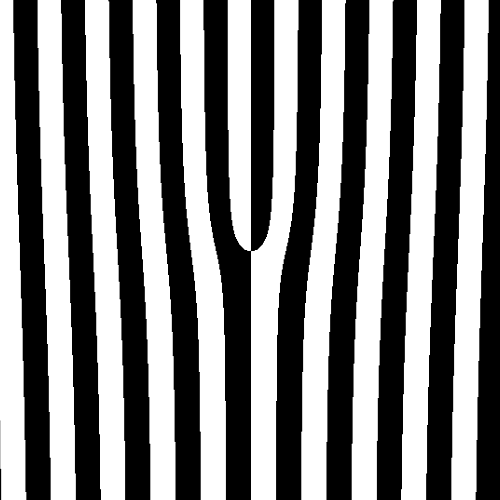
\includegraphics[width=0.75\marginparwidth]{illustrations/tomography/fork-hologram}
\caption{Typical design of a fork hologram with vortex charge 2.}
\label{tomography:fig:fork-hologram}
\end{marginfigure}

A $4f$\ lens system transports the beam to the back focal plane of a microscope objective, which focuses the far field of the beam onto the sample, down to a size of several microns. On its way, the beam passes through a half-wave plate which allows the experiment to be conducted with any desired linear polarization.

The sample (Fig.~\ref{tomography:fig:sample}) consists of a gold film, $200\unit{nm}$ thick, attached to a glass substrate by a $10\unit{nm}$ titanium adhesion layer.
The strongly dissipative titanium layer ensures that surface plasmons can only propagate on the gold-air interface \cite{Schouten2005}. The sample contains pairs of double slits, which are ion-beam milled through the gold. The slits used in this experiment are all $50\micron$ long and $100\unit{nm}$ wide, and the pairs are separated by $25$, $50$, and $75\micron$. For comparison, the damping length of surface plasmons on gold at this wavelength is around $50\micron$. We illuminate the emitter slit with our vortex beam and image the light emerging from the receiver slit onto a \gls{CCD} camera. The incident beam is polarized so as to couple optimally with surface plasmons.%
%
\begin{marginfigure}
\forcerectofloat
\import{illustrations/tomography/}{illustrations/tomography/sample.pdf_tex}
\caption{Sketch of a typical nanostructure on the sample.
The slits are 100 nm wide and 50 \textmu m long, and separated by 25, 50, or 75 \textmu m.}
\label{tomography:fig:sample}
\end{marginfigure}

We illuminate the emitter slit with the beam, causing it to launch a surface plasmon wave along the gold-air interface towards the receiver slit.\footnote{The emitter also launches a wave in the other direction, but we do not detect this wave.}
Its amplitude at the emitter is given by the local field amplitude incident on the slit. In between the slits, the wave diffracts freely. The receiver slit scatters the diffracted plasmonic field into free space.
The diffraction pattern contains information on both the phase and the amplitude of the light incident on the emitter slit.

\begin{figure}[tb]
\forceversofloat\centering
\import{illustrations/tomography/}{illustrations/tomography/double-slit-cartoon.pdf_tex}
\caption{Close-up sketch of the tomography process.
A vortex beam, with a ring-shaped transverse intensity profile, is incident on the emitter slit.
The slit scatters the incident light, launching surface plasmons, proportional to the field amplitude (which is very low inside the ring.)
The surface plasmons propagate to the receiver slit and are scattered into free space.}
\label{tomography:fig:cartoon}
\end{figure}
%
The sample is mounted so as to allow translation transverse to the optical axis. At the start of a measurement, the beam is incident to one side of the slit pair. We translate the sample along the positive $z$-axis in $100\unit{nm}$ increments so that the emitter slit travels through the beam. At each position of the sample, we record the intensity profile of the light scattered from the receiver slit. We then assemble these profiles together in a tomogram, so that each vertical slice of the tomogram corresponds to one slice of the incident vortex beam after propagation from emitter to receiver.
Figure~\ref{tomography:fig:cartoon} shows a sketch of the tomography process.

We calculate the expected tomograms by modelling the emitter slit as a plasmonic line source with its field amplitude given by the incident vortex beam's free-space field amplitude at that point on the sample. We then calculate the evolution of this field under propagation from emitter to receiver, using the Fresnel-Kirchhoff diffraction integral, modified for surface plasmons \cite{Teperik2009}. We model the receiver slit as another line, which scatters light into free space proportional to the plasmonic amplitude it receives.

\section{Tomograms}

\begin{figure}[tb]
\forcerectofloat\centering
\includegraphics{graphs/tomography/charge}
\caption{Calculated (a--c) and experimental tomograms (d--f) for beams on slits separated by $25\micron$, with vortex charge $Q = +1$ (a and d), $Q = -1$ (b and e), and $Q = -3$ (c and f).
Note that the intensity zeroes in (c) and (f) occur nicely along a straight line.}
\label{fig2}
\end{figure}%
%
\sectionstart{Figure~\ref{fig2} shows} the calculated and measured tomograms for incident beams of vortex charge $Q = +1$, $-1$, and $-3$, respectively, using slits separated by $25\micron$. The tomographic patterns are very different from the original ring-shaped vortex beams. First, the pattern is no longer rotationally symmetric, but has a two-fold symmetric, elongated shape. Second, the patterns for beams with vortex charge $Q = +1$ and $Q = -1$ are each other's mirror image. Third, the orientation of the long axis of the pattern carries the sign of the vortex charge. Finally, the magnitude of the vortex charge can be read off directly from the number of spatially separated intensity zeroes in the pattern. Our calculations, which are in excellent agreement with our experimental results, indicate that these intensity zeroes correspond to phase vortices in the tomogram.

Figure~\ref{fig3} shows calculated and measured tomograms for a $Q = -1$ incident beam for slit pairs with increasingly larger separations. As the distance between the slits increases, the tomographic pattern remains essentially the same but spreads out more, approaching Fraunhofer diffraction of the surface plasmons.
%
\begin{figure}[tb]
\forceversofloat\centering
\includegraphics{graphs/tomography/distance}
\caption{Calculated (a--c) and experimental tomograms (d--f) for a $Q = -1$ vortex beam on slits separated by distances of $25\micron$ (a and d), $50\micron$ (b and e), and $75\micron$ (c and f).}
\label{fig3}
\end{figure}

\section{Interpretation}

\sectionstart{There is an intuitive way of explaining} why the observed tomographic patterns look as they do.
The surface plasmon field amplitude at the emitter slit diffracts as the plasmons travel from the emitter to the receiver.
We can consider the field's amplitude at the emitter equivalent to an amplitude mask in a screen, with bright areas corresponding to slits.
The screen is illuminated from behind by a plane wave at an angle determined by the field's phase at the emitter.
If we place a second screen at some distance, corresponding to the receiver, then the positions of the bright and dark spots in the tomogram follow directly by considering where constructive and destructive interference occur on the second screen.

\begin{figure}[tb]
\forceversofloat\centering
\includegraphics{graphs/tomography/diffraction}
\caption{(a) Calculated intensity pattern of a $Q = -3$ vortex beam.
Three important cross sections are indicated by vertical lines.
(b) Calculated tomogram for a $Q = -3$ vortex beam on slits separated by $25\micron$ (cf.\ Fig.~\ref{fig2}c). The indicated cross sections are identical to those of Fig.~\ref{fig4}a. Local minima and maxima in the tomograms are marked by $\times$ and \textopenbullet, respectively.
These marks correspond to those in the diffraction patterns depicted schematically in Figs.~\ref{tomography:fig:single-slit}, \ref{tomography:fig:double-slit-inphase}, and \ref{tomography:fig:double-slit-antiphase}.}
\label{fig4}
\end{figure}
%
We discuss the $Q = -3$ case in some detail with the aid of Fig.~\ref{fig4}. In Fig.~\ref{fig4}a we depict the intensity pattern of the incident beam at the surface of the gold film; it is intersected by three vertical lines labeled 1, 2 and 3, corresponding to three different positions of the emitter slit. In Fig.~\ref{fig4}b we show the tomogram of the $Q = -3$ beam, with the equivalent three positions of the receiver slit.
Line 1 is tangent to the ring of maximum intensity of the $Q=-3$ input beam.
In the tomogram, the intense diffraction spot along line 1 corresponds to the case that the emitter slit picks up an essentially single-spot intensity distribution with a slanted phase front, arising from the azimuthal phase dependence of the incident beam. The corresponding diffraction pattern is that of a plane wave incident at an angle through a single slit: a single off-axis spot results (see Fig.~\ref{tomography:fig:single-slit}).
%
\begin{marginfigure}
\centering
\import{illustrations/tomography/}{illustrations/tomography/single-slit-oblique.pdf_tex}
\caption{Diffraction pattern of light at a single slit under oblique incidence.
Corresponds to line 1 in Fig.~\ref{fig4}.}
\label{tomography:fig:single-slit}
\end{marginfigure}%

When the emitter slit is positioned more towards the center of the incident beam, along line 2, the generated plasmonic field is bimodal with a dip between the intensity maxima. In this region the phase of the plasmonic field varies steeply and linearly with position along the emitter slit. At this particular position of this slit, the relative phase of the two maxima of the bimodal intensity distribution equals $2\pi$. Conceptually, the plasmonic diffraction pattern should therefore be similar to the pattern arising from a double slit illuminated at an angle in such a way that the two slits have equal phase, up to a factor $2\pi$ (see Fig.~\ref{tomography:fig:double-slit-inphase}).
%
\begin{marginfigure}
\forcerectofloat\centering
\import{illustrations/tomography/}{illustrations/tomography/double-slit-inphase.pdf_tex}
\caption{Diffraction pattern of light at a double slit under oblique incidence, such that the local field at the slits is in phase.
Corresponds to line 2 in Fig.~\ref{fig4}.}
\label{tomography:fig:double-slit-inphase}
\end{marginfigure}

Finally, when the emitter slit is at line 3, the center of the incident beam, the plasmonic field will again be bimodal, now with a phase difference of $3\pi$. The diffraction pattern at the receiver slit will be double-slit-like with a zero in the center as a result of destructive interference (see Fig.~\ref{tomography:fig:double-slit-antiphase}).
%
\begin{marginfigure}
\centering
\import{illustrations/tomography/}{illustrations/tomography/double-slit-antiphase.pdf_tex}
\caption{Diffraction pattern of light at a double slit in antiphase.
Corresponds to line 3 in Fig.~\ref{fig4}.}
\label{tomography:fig:double-slit-antiphase}
\end{marginfigure}

\section{Non-integer vortex experiment}

\sectionstart{In order to consider} the application of this method to more complex vor\-tex-car\-ry\-ing fields, we also conducted experiments with a non-integer vortex beam, using a spiral phase plate \cite{Oemrawsingh2004b} to generate the desired field with vortex charge $Q=3\half$.
Figure~\ref{tomography:fig:spp} is a sketch of a spiral phase plate.
The far-field diffraction pattern of such a beam is not rotationally symmetric, so we oriented the phase plate to produce an incident intensity pattern as shown in Fig.~\ref{fig5}a, with the slits oriented vertically. The incident pattern shows three close-lying, separated $Q = +1$ vortices in the center, with an additional one intruding from the bottom.
Figures~\ref{fig5}b and \ref{fig5}c show two measured tomograms at different slit separations, while Figs.~\ref{fig5}d and \ref{fig5}e show the corresponding calculations.
These tomograms are devoid of any symmetry.
Specifically, the three vortices are not arranged along a straight line, unlike the integer-vortex case.
They also show a fourth vortex intruding from the side, although the visibility of the fourth vortex in the measurements is somewhat marginal.
Currently we do not account for any inhomogeneity in the slit width; this problem might be solved by using a ptychographical algorithm, which iteratively reconstructs a field's complex amplitude, and the transfer function of the object used to probe it \cite{Maiden2009}.
%
\begin{marginfigure}
\centering
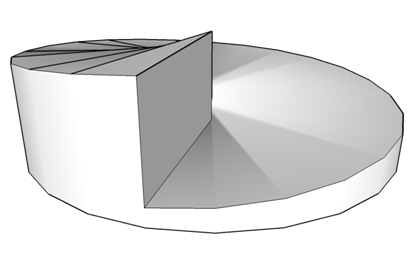
\includegraphics[width=1.37in]{illustrations/tomography/spp} % max width @300dpi
\caption{Sketch of a typical spiral phase plate.}
\label{tomography:fig:spp}
\end{marginfigure}
%
\begin{figure*}[tb]
\forceversofloat\centering
\includegraphics{graphs/tomography/halfvortex}
\caption{(a) Far-field diffraction pattern of a $Q = +3\half$ vortex beam; (b) experimental tomogram of this beam on slits separated by 25 \textmu m; (c) 75 \textmu m; (d) calculated tomogram of an ideal $Q=+3\half$ vortex beam on slits separated by 25 \textmu m; (e) 75 \textmu m.
Three intensity nodes are visible, but they are not arranged along a straight line.}
\label{fig5}
\end{figure*}

For a better understanding of the relation between the fractional part of the vortex charge and the presence and position of the fourth vortex in the tomogram, we calculated the tomograms of beams with various vortex charges between $+3$ and $+4$, shown in Fig.~\ref{tomography:fig:fractional}.
We see that as $Q$ increases, the fourth vortex, as seen in Fig.~\ref{fig5}, approaches the three existing vortices, and eventually joins them in a straight line at $Q=+4$.
The vortices are arranged in a straight line only when $Q$ is an integer.
This suggests that a non-integer vortex charge can be determined from the deviation of the vortices' arrangement from a straight line, the angle of which is determined mainly by the ratio of the distance between the slits to the spot size of the beam.
Our calculations indicate that any dependence on $Q$ is less than 1\textdegree\ and may be a numerical artifact.
%
%%%%% TWEAK %%%%%%%%%%%%%%%%%%%%%%%%%%%%%%%%%%%
\begin{figure*}[b]
\centering
\includegraphics{graphs/tomography/charge-evolution}
\caption{Calculated tomograms of vortex beams with $Q$ ranging from $+3$ to $+4$ on slits separated by 50 \textmu m.
(a) $Q=+3$; (b) $Q=+3\boxfrac{1}{4}$; (c) $Q=+3\half$; (d) $Q=+3\boxfrac{3}{4}$; (e) $Q=+4$.
The locations of the intensity zeroes are indicated with dots.
In (a) and (e), the size of the original vortex ring is superimposed on the tomogram.}
\label{tomography:fig:fractional}
\end{figure*}

\section{Summary}

\sectionstart{We have used the diffraction} of surface plasmon polaritons to analyze a vortex-carrying light beam slice by slice, in order to recover information about the beam's phase: specifically, its vortex charge.
Although the determination of non-integer vortex charges is not possible at a glance, we have shown through calculations that the magnitude of a non-integer vortex charge may be determined by measuring how much the arrangement of the vortices deviates from a straight line.

Phase retrieval normally requires some technique such as interferometry or a combination of near-field and far-field measurements. The current experiment's two slits can be considered to measure the surface plasmons' near field and far field. Therefore, the technique might be generalized to phase retrieval of arbitrary fields.
Also, the sample's small size and the small distances between the optics involved suggest that the experiment can be easily miniaturized.
Therefore, it has a potential application as a wavefront sensor.
